
\section[Miscellaneous]{Miscellaneous}
\label{sec:misc}
\addcontentsline{toc}{section}{\thesection. Miscellaneous}


\subsection[Multinomial Logistic Regression]{Multinomial Logistic Regression}
\label{sec:multinom}
\addcontentsline{toc}{subsection}{\thesubsection. Multinomial Logistic Regression}


\code{fitMultinom()} is a utility function which can fit an ROC model with
$\phi$ values, assuming no measurement errors as in~\citet{Shah2011}.
A typical usage is:
\begin{Code}
> demo(fitMultinom, 'cubfit')
\end{Code}
or
\begin{Code}
library(cubfits, quietly = TRUE)

# fit Shah & Gilchrist (2011)
init.function(model = "roc")
fitlist <- fitMultinom(ex.train$reu13.df, ex.train$phi.Obs,
                       ex.train$y, ex.train$n)
ret.fit <- prop.model.roc(fitlist, phi.Obs.lim = range(ex.train$phi.Obs))
aa.names <- names(ex.train$reu13.df)

# plot.
par(mfrow = c(1, 3))
for(i.aa in 1:length(aa.names)){
  plotmodel(ret.model = ret.fit[[i.aa]], main = aa.names[i.aa])
}
\end{Code}
where \code{fitlist} is an object of \code{b} data structure containing
all estimations of $(log(\mu), \Delta t)$ for each synonymous codon and
amino acid.
This is a quick fit assuming no measurement error on expression levels.
This demo returns plots in Figure~\ref{fig:fitMultinom}
\begin{figure}[ht]
\centering
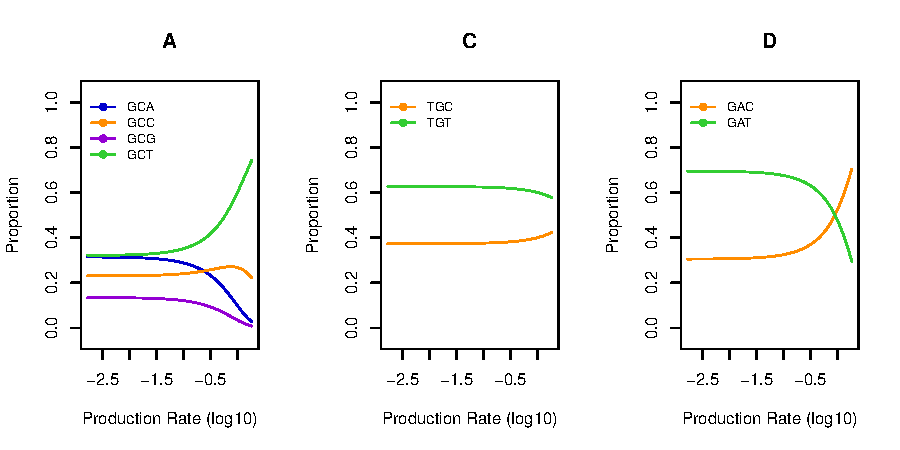
\includegraphics[width=6in]{cubfits-include/figure/fitMultinom}
\caption{A simple prediction plot, similar to Figure~\ref{fig:plotbin}
except empirical binning.
}
\label{fig:fitMultinom}
\end{figure}

{\color{red} \bf Important:}
Note that \code{init.function(model = "roc")} initializes generic functions
for the ROC model and \code{fitMultinom()} can access corresponding generic
functions from the \code{.cubfitsEnv} environment. The generic function then
performs multinomial logistic regression on the input summarized statistics,
and \code{VGAM::vglm()} can fit and return parameter estimations.
Therefore, there is only need to initialize once before MCMC iterations, such as
the three main function in Section~\ref{sec:main_functions}. For performance
issues, all calls within MCMC iterations should access generic functions, such
as via \code{.cubfitEnv$fitMultinom()} regardless of the model. Do \textbf{NOT}
access \code{fitMultinom()} within any MCMC iteration.




\subsection[Asymmetric Laplace Distribution]{Asymmetric Laplace Distribution}
\label{sec:asl}
\addcontentsline{toc}{subsection}{\thesubsection. Asymmetric Laplace Distribution}

As with the regular \proglang{R} functions for different distributions 
(\code{dnorm()}, \code{pnorm()}, etc.),
\pkg{cubfits} provides analogous functions for asymmetric Laplace distribution
(ASL) such as \code{rasl()}, \code{dasl()}, \code{pasl()}, and \code{qasl()}.
See \citep{KKP2001} for more details about the ASL distribution.
Finding a MLE numerically is possible for ASL random samples and
is implemented in the \code{asl.optim()}.

For example,
Yassour dataset~\citep{Yassour2009} has 6303 gene expression measurements and
four replicates.
I took the geometric averaged mean of the replicates for each gene and
fitted the ASL model to the means of 6303 genes as suggested
by~\cite{Wallace2013}.
The data distribution and the ASL fits are shown
in Figures~\ref{fig:asl} which can be done as the next.
\begin{Code}
> demo(yassour.asl, 'cubfits')
\end{Code}

Further, I also used normal mixture models to fit the same data using the EM
algorithm implemented in the \pkg{EMCluster}~\citep{EMCluster} package.
Figure~\ref{fig:mixture} shows the fits
for $K = 1, 2,\ldots, 6$ components of normal mixture models,
which can be done via a call to
\begin{Code}
> demo(yassour.mixture, 'cubfits')
\end{Code}

Table~\ref{tab:asl_mixture}
provides some details for model comparison. Note that $K=6$ has
a smaller log likelihood than $K=5$.  This means that the EM algorithm
converges to local optimum and may indicate an overestimated number of
components. $K = 4$ is the best choice among all models by the smallest
BIC.

\begin{figure}[h]
  \centering
  \begin{subfigure}[b]{.45\textwidth}
    \centering
    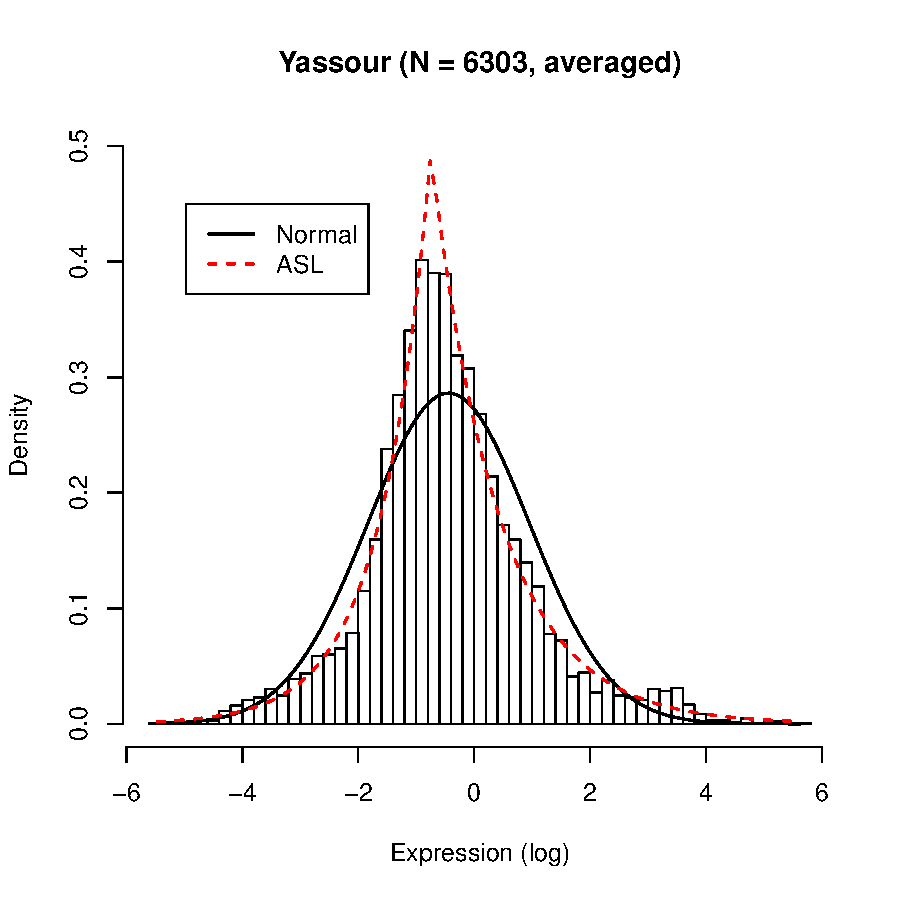
\includegraphics[height=7.5cm,width=7.5cm]{cubfits-include/figure/more_asl}
    \caption{ASL model}
    \label{fig:asl}
  \end{subfigure}
  \begin{subfigure}[b]{.45\textwidth}
    \centering
    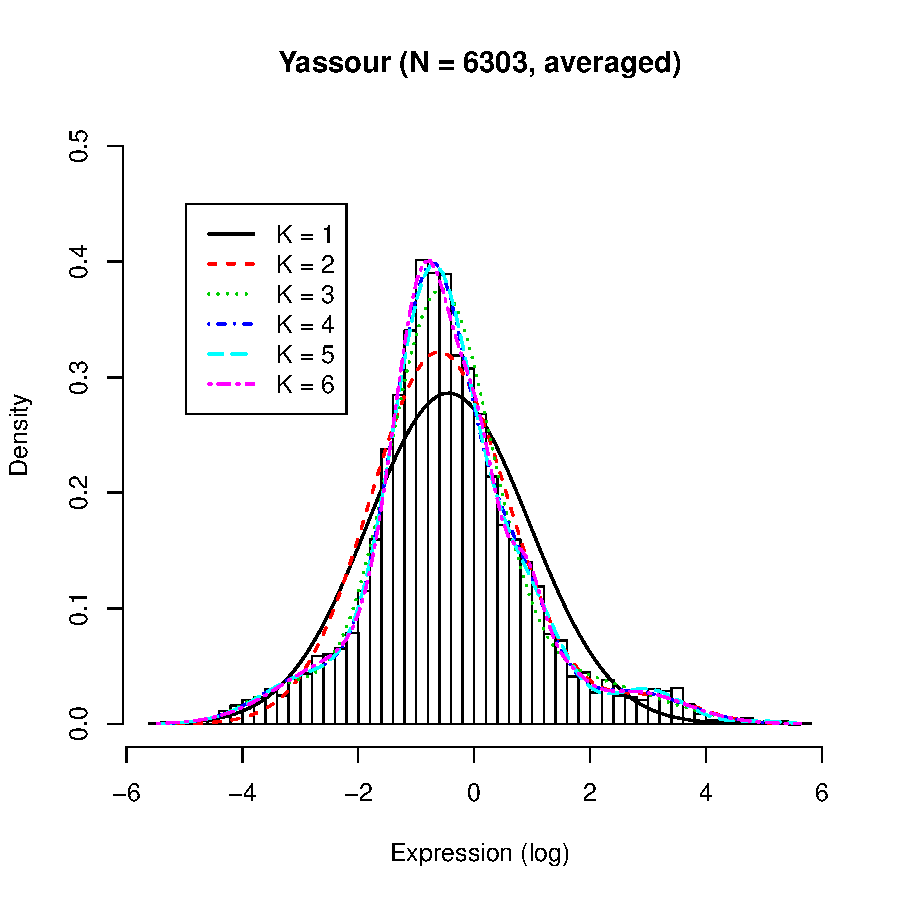
\includegraphics[height=7.5cm,width=7.5cm]{cubfits-include/figure/more_mixture}
    \caption{Mixture normal model}
    \label{fig:mixture}
  \end{subfigure}
  \caption{Different distribution fits to Yassour dataset.}
  \label{fig:asl_mixture}
\end{figure}

\begin{table}[h]
  \centering
  \begin{tabular}{ccccc} \hline\hline
  Model & $p$  & $\log L$    & $AIC$      & $BIC$ \\ \hline
  ASL   & $3$  & $-10739.84$ & $21485.68$ & $21505.93$ \\
  Normal /
  $K=1$ & $2$  & $-11033.55$ & $22071.10$ & $22084.60$ \\
  $K=2$ & $5$  & $-10820.47$ & $21650.93$ & $21684.68$ \\
  $K=3$ & $8$  & $-10687.06$ & $21390.12$ & $21444.11$ \\
  $K=4$ & $11$ & $-10655.55$ & $21333.10$ & $21407.34$ \\
  $K=5$ & $14$ & $-10649.69$ & $21327.38$ & $21421.87$ \\
  $K=6$ & $17$ & $-10653.19$ & $21340.38$ & $21455.11$ \\
  \hline\hline
  \end{tabular}
  \caption{$K$ is the number of components for the mixture normal model
           and $K=1$ is equivalent to normal model.
           $p$ is the number of parameters for the fitted model,
           $\log L$ is the log likelihood, $AIC = -2 \log L + 2p$, and
           $BIC = -2 \log L + p\log(n)$ where $n = 6303$ is
           the number of samples.}
  \label{tab:asl_mixture}
\end{table}
